\documentclass[a4paper,10pt,oneside]{article}
\usepackage[polutonikogreek,italian]{babel}
\usepackage[utf8x]{inputenc}
\usepackage{amsmath}
\usepackage{amsthm}
\usepackage{amssymb}
\usepackage{amscd}
\usepackage[pdftex,colorlinks=true,urlcolor=black]{hyperref}
\usepackage{graphicx}
\usepackage{float}
\usepackage{array}
\usepackage{rotating}
\usepackage[small]{caption}
\usepackage{lscape}
\usepackage{fancybox}
\usepackage{booktabs}
\usepackage[noanswer]{exercise}
\parindent0ex
\renewcommand{\fboxsep}{0.4cm}
\renewcommand{\textfraction}{0.05}
\renewcommand{\topfraction}{0.95}
\renewcommand{\bottomfraction}{0.95}
\renewcommand{\floatpagefraction}{0.35}
\renewcommand{\ExerciseName}{Esercizio}
\renewcommand{\ExerciseListName}{Es}
\setcounter{totalnumber}{5}
\restylefloat{figure}
\begin{document}
\section*{Il moto e le sue cause}
\begin{figure}[H]
 \centering
 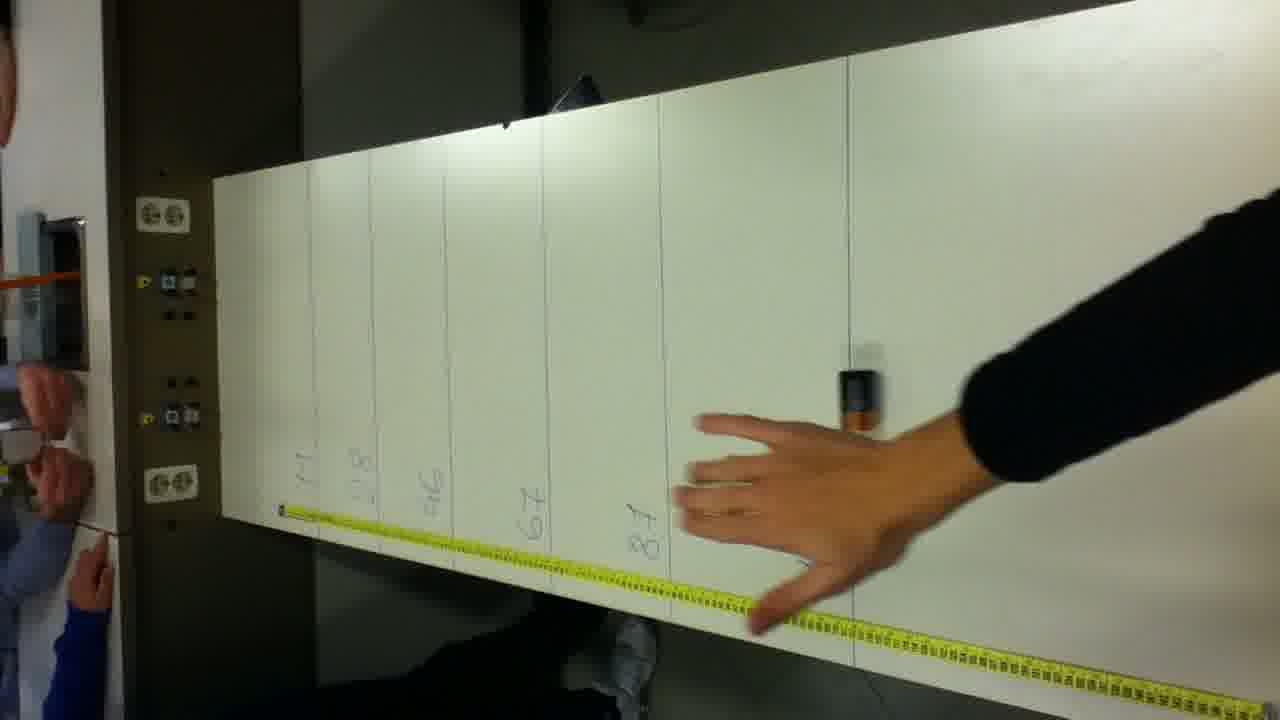
\includegraphics[width=.7\textwidth]{../immagini/lancio.jpeg}
 % podista.png
 \label{fig:lancio della batteria}
\end{figure}

La conoscenza dei concetti di spazio, velocità e accelerazione è una premessa fondamentale per lo studio della fisica, perché i fenomeni naturali sono eventi dinamici di cui è necessario saper analizzare i mutamenti.\newline
Però la fisica si pone un obiettivo più alto, che trascende la cinematica. Non è sufficiente, infatti, riconoscere le caratteristiche di un fenomeno, ma è necessario sviluppare la capacità di ricavare {\bf le cause} di ciò che si osserva.\newline

In questo capitolo, partendo dall'osservazione di un fenomeno cinematico estremamente semplice, cercheremo di distinguere il ruolo della gravità e dell'attrito come cause del moto e riflettere su alcuni caratteri dello scivolamento lungo un piano inclinato.\newline

Siccome la trattazione si appoggia a un'attività di laboratorio realmente svolta in una scuola superiore, quanto segue sarà esposto, in alcune parti, secondo la forma documentale della relazione di laboratorio.

\subsubsection*{Il rotolamento di un cilindro}

Come mostra l'immagine in apertura di capitolo, l'attività su cui è basata questa unità didattica riguarda il rotolamento di un cilindro (nello specifico una pila commerciale) lungo un banco di un laboratorio di fisica e descrive un esperimento realmente realizzato in una scuola superiore.\newline

Il banco era liscio e aveva la lunghezza di un paio di metri. La pila è stata fatta rotolare più volte, con spinte diverse. {\slshape Sorprendentemente}, in ogni lancio, il movimento della pila si è prolungato al di là di ogni attesa, terminando sulla parete in fondo al tavolo, anche nei casi in cui la velocità iniziale era molto piccola, dando quasi la sensazione che il moto della potesse prolungarsi all'infinito.\newline
Allora abbiamo provato a spingere la pila nella direzione opposta, dalla parete verso il lato libero del tavolo. Il moto è apparso estremamente diverso: adesso la pila rallentava visibilmente e di solito si fermava sul banco. Era proprio necesario imprimere una spinta molto robusta per riuscire a percorrere l'intera lunghezza del tavolo.\newline

Dove aver eseguito un certo numero di esperienze, ci siamo disposti a documentarle utilizzando un foglio suddiviso un foglio in tre colonne corrispondenti alle voci seguenti:\newline

\begin{center}
\begin{tabular}{|c|c|c|}
\hline
{\bf Cosa faccio} &{\bf Cosa osservo }&{\bf Come spiego }\\
\hline
\end{tabular}
\end{center}


\subsubsection*{Osservazioni preliminari}
L'abitudine a documentare ordinatamente le osservazioni è una abilità molto importante, perché da essa discende la validità formale dell'attività di ricerca, che è alla base del {\bf metodo scientifico sperimentale}.\newline

Qui riportiamo, ma volutamente in ordine sparso, alcune delle osservazioni che sono state formulate durante la discussione, dando compito al lettore di collocarle opportunamente nelle tre colonne.\newline

Il piano è inclinato.\newline
Il piano è leggermente inclinato, anche se la pendenza è impercettibile.\newline
La pila si muove in modo uniforme.\newline
Il piano è liscio.\newline
La pila rallenta durante la salita.\newline
Il piano è ruvido e fa attrito.\newline
La gravità accelera il moto.\newline
La gravità rallenta la pila.\newline
La velocità del moto aumenta ma di pochissimo.\newline
Se la spinta iniziale è molto piccola si osserva una piccola accelerazione.\newline


\subsubsection*{La descrizione strumentale}

Non tutte le osservazioni preliminari effettuate immediatamente risultavano concordi. Alcune, addirittura, erano in piena contraddizione. Abbiamo perciò sentito la necessità di individuare degli strumenti di misura capaci di fornire dei dati oggettivi affidabili.\newline

Abbiamo perciò deciso di riprendere il movimento facendo uso delle webcam dei nostri computer portatili o dei nostri cellulari, per realizzare successivamente un'analisi in laboratorio di informatica.\newline

Inizialmente, abbiamo disposto un metro da sarta centimetrato lungo il banco, ma ci siamo accorti che la lettura sulle telecamere risultava piuttosto incerta, a causa della bassa risoluzione del metro, o forse a causa della nostra limitata perizia di cameramen. Di conseguenza, abbiamo preferito tracciare sul banco alcune linee trasversali con dei pennarelli non indelebili.

I filmati sono stati scaricati in laboratorio di informatica e scomposti in fotogrammi con l'uso del programma libero ffmpeg.\newline
Per ogni filmato è stata creata una apposita cartella di fotogrammi, numerati in ordine cronologico. Individuando il numero dei fotogrammi in cui la pila toccava le linee trasversali, era possibile ottenere dei grafici spazio tempo che sono stati successivamente analizzati con geogebra.

\subsection*{L'analisi dei dati}
\subsection{Moto in discesa}
In questo paragrafo vogliamo analizzare due grafici particolari che sono stati ottenuti da alcuni studenti, come esempio di come può essere condotta l'analisi dei dati di un esperimento.

 Questo è l'aspetto di uno dei grafici:

\begin{figure}[H]
 \centering
 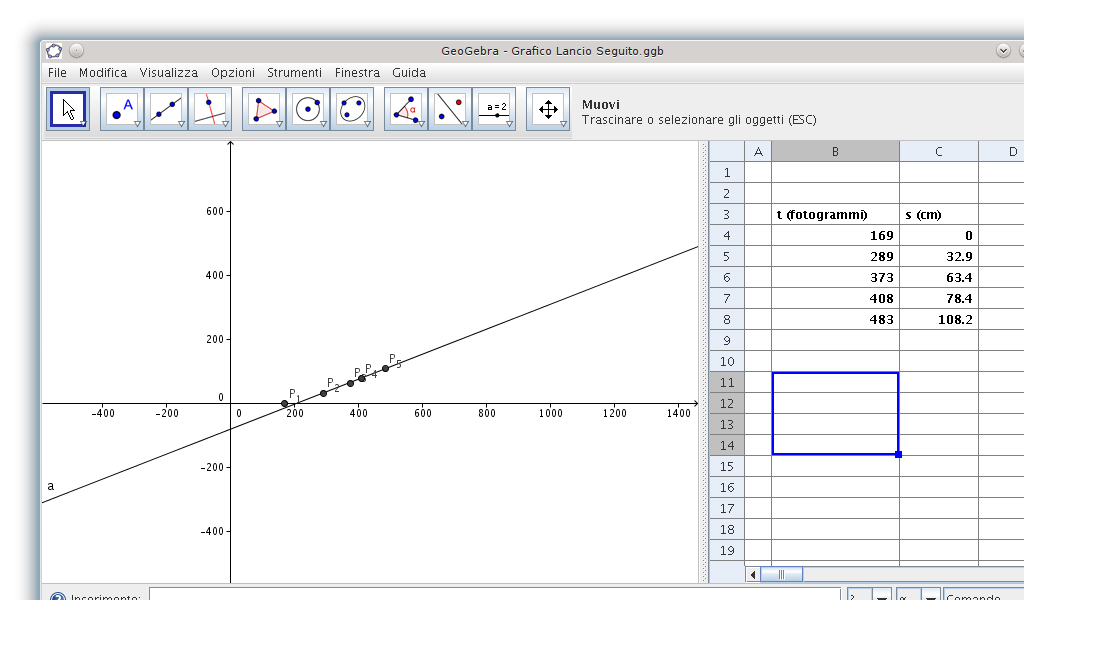
\includegraphics[width=.7\textwidth]{../immagini/discesa.png}
 \label{fig:moto di discesa}
\end{figure}

Come si osserva, quasi tutti i dati sono allineati su una retta ben riconoscibile.\newline
Solo uno dei punti si discosta visibilmente dalla retta.\newline

Per esercizio, valutate le veocità medie per ciscuna coppia di punti sperimentali e valutate se sono tutte uguali tra loro.\newline

La retta tracciata sul grafico non costituisce un rilievo sperimentale, ma una elaborazione realizzata da alcuni studenti sulla base dei dati acquisiti. Per ricavarla, è stato semplicemente estratto un valore credibile per il coefficiente angolare ed imposta la condizione di passaggio per un punto. Un gruppo di studenti più avanzato avrebbe potuto applicare ai dati delle tecniche rigorose di regressione lineare, ma in questo caso, probabilmente, non serve troppa matematica per dare un'intrepretazione fisica accettabile del fenomeno.\newline

Una possibile interpretazione dei dati può essere la seguente:
\begin{center}
\begin{tabular}{||*{3}{p{5cm}|}|}
\hline
Cosa faccio & Cosa osservo & Come spiego \\
\hline
Una pila viene lanciata lungo un piano inclinato con una velocità iniziale modesta. &
La pila accelera per un breve tratto iniziale, ma successivamente si stabilizza in un moto a velocità costante per un tempo piuttosto lungo, che si arresta solamente sulla parete di fondo. &
L'accelerazione iniziale potrebbe far pensare ad una leggera inclinazione del banco, che successivamente scompare o viene equilibrata da qualche altro effetto non facilmente individuabile. \\
\hline
\end{tabular}
\end{center}

\subsection{Moto in salita}
Questo è un secondo grafico:

\begin{figure}[H]
 \centering
 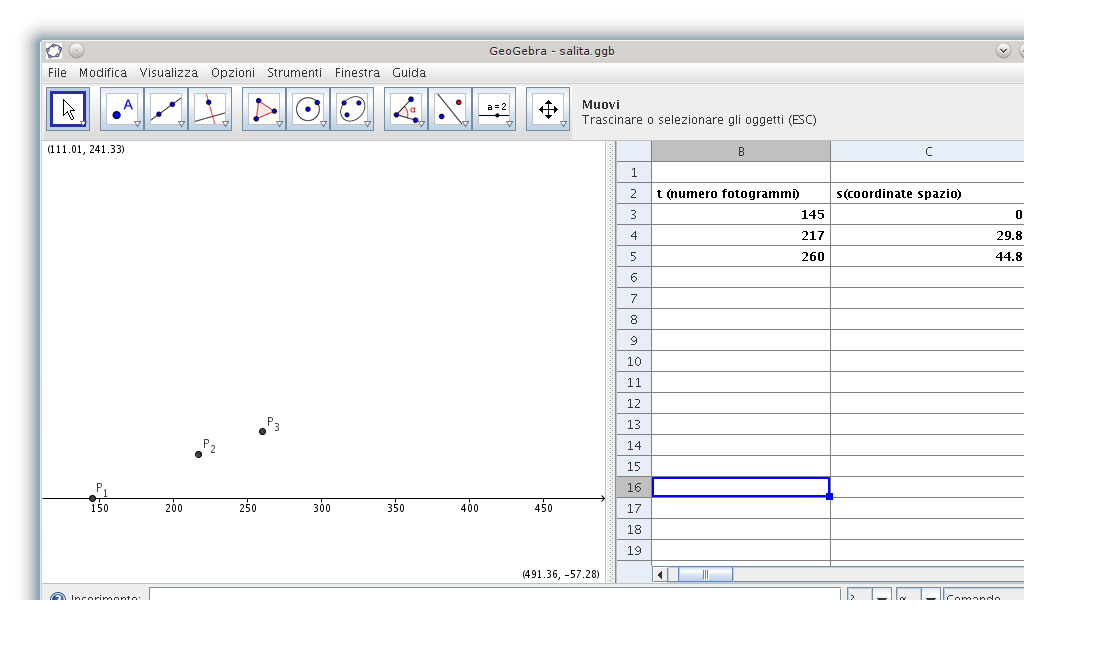
\includegraphics[width=.7\textwidth]{../immagini/salita.png}
 \label{fig:moto di salita}
\end{figure}

È relativo a un lancio della batteria all'indietro. Tutte le volte in cui la batteria è stata lanciata all'indietro, è stata osservata, anche ad occhio nudo, una accelerazione negativa, come se il percorso fosse in leggera salita.

I nostri dati, in questo caso, contengono appena tre punti. Ma questo è il minimo indispensable per distinguere un moto uniforme da uno accelerato.\newline
In effetti il punto $ P_3 $ è troppo basso per essere allineato e il calcolo delle velocità medie indica un rallentamento.\newline

Usando questi tre punti, possiamo valutare l'{\bf accelerazione media} della batteria.\newline
Questo equivale ad assumere che l'equazione del moto corrisponda all'equazione del moto uniformente accelerato:
\begin{center}
  \begin{equation}
  	s = \frac{1}{2} a t^2 + v_0 t + s_0
  \end{equation}
\end{center}

Sostituendo alle variabili $s$ e $t$ le coordinate dei punti $P_1$, $P_2$ e $P_3$, si ottiene un sistema lineare che restituisce i valori dei parametri $a$, $v_0$ e $s_0$.\newline
Volendo, ci si può aiutare con un programma grafico, capace di calcolare l'equazione di una parabola per tre punti e di rappresentarla su un grafico. Qui sotto, mostriamo un'immagine prodotta con kig:

\begin{figure}[H]
 \centering
 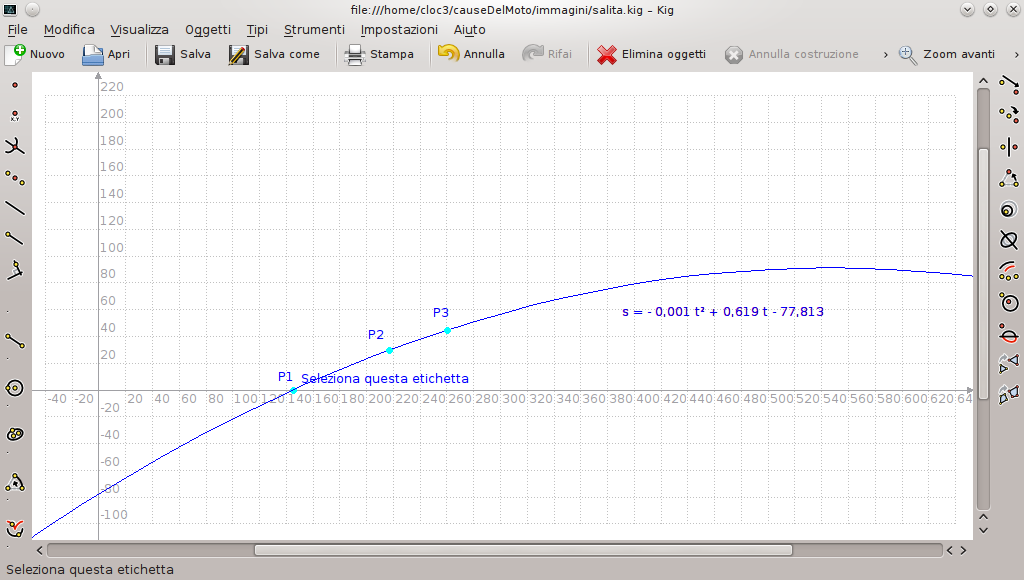
\includegraphics[width=.7\textwidth]{../immagini/salitaConKig.png}
 \label{fig:parabolaPerTrePunti}
\end{figure}

\subsection{Le unità di misura}

Elaborare dei dati non si esaurisce semplicemente nell'uso di programmi grafici che rappresentano i dati acquisiti. È estremamente importante, invece, mantenere il controllo di ciò che i dati significano, cominciando dalla valutazione delle unità di misura. Nel lavoro che stiamo analizzando, i tempi sono determinati dal numero di fotogramma acquisito dalla webcam. L'intervallo di tempo che separa un fotogramma dall'altro è una piccola frazione di secondo.\newline
Le nostre telecamere acquisivano 30 fotogrammi al secondo.\newline

Le lunghezze, invece, sono state acquisite in centimetri. Se desideriamo esprimere le nostre accelerazioni in metri e secondi, dobbiamo considerare che:
\begin{center}
\begin{math}
1 \frac{cm}{{fotogramma}^2}=1 \frac{10^{-2}m}{{(30^{-1}}s)^2} = 9 \frac{m}{s^{-2}}
\end{math}
\end{center}

Osserviamo anche che il programma kig produce una stima dell'accelerazione con una sola cifra significativa, che è riduttiva per la precisione con la quale abbiamo raccolto i notri dati. Questa sezione, relativa alla elaborazione dei dati, può quindi assumere gradi diversi di approfondimento, che sono lasciati alla determinazione dell'insegnante.

\subsubsection*{Comprendere i dati: il ruolo della gravità e dell'attrito}

La produzione e l'analisi dei filmati offre permette di allargare molto l'osservazione,  controllando numericamente molti particolari, tuttavia una comprensione approfondita di una fenomenologia richiede una attività di sintesi che, fino a questo monento non è ancora compiuta.\newline

Riprendendo lo schema a tre colonne: "Cosa faccio", "Cosa osservo", "Come spiego", si può riconoscere facilemente che l'ultima delle tre colonne, fino ad ora, non è stata sviluppata in modo esaustivo.\newline
Probabilmente, l'unica con conclusione che, al momento, viene spontaneo acquisire è che il piano del banco non è perfettamente orrizzontale, a causa delle differenze osservate nel moto di discesa e quello di salita.\newline

Tuttavia, i grafici possono dire qualcosa in più. Perché il moto in salita è un moto accelerato, mentre quello in discesa è quasi perfettamente costante. Quali sono le {\bf cause} che determinano l'accelarazione o il moto uniforme?\newline

L'inclinazione del piano, ad esempio, non è sufficiente. Possiamo accettare che la pila sia frenata per gravità in salita, ma dovremmo aspettarci, durante la discesa, una accelerazione uguale e contraria. Se invece il moto è uniforme, significa che il sistema è affetto da qualche causa di accelerazione differente. In effetti, sebbene la pila sia un oggetto cilindrico, è frenata da qualche forma di attrito. Anzi, a pensarci bene, se non ci fosse un attrito non potrebbe neppure rotolare, ma traslerebbe rigidamente come un oggetto in volo libero sopra il tavolo. La rotazione, di conseguenza, è possibile solo se il piano funge da punto di appoggio per il cilindro.\newline

Possiamo affermare, dunque, che gli elementi necessari per descrivere le cause del moto della pila sono:\newline
\begin{itemize}
\item {la velocità;}
\item {la accelerazione verso il basso, associata alla gravità;}
\item {la decelerazione di attito, opposta alla velocità;}
\end{itemize}

Trattandosi di grandezze vettoriali possono essere rappresentate graficamente in questo modo:

\begin{figure}[H]
 \centering
 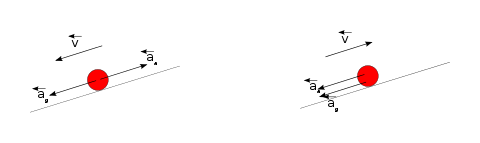
\includegraphics[width=.7\textwidth]{../immagini/leCauseDelMotoDellaPila.png}
 \label{fig:causeDelMotoDellaPila}
\end{figure}

Dalla figura, possiamo osservare che i fattori che determinano il comportamento della pila, cioè la gravità e l'attrito, si sovrappongono in modo differente durante la salita e durante la discesa, e questo può spiegare perché uno dei moti è accelerato mentre l'altro no. Adesso siamo in grado di riscrivere il nostro schema a tre colonne in un modo migliore che in precedenza:

\begin{center}
\begin{tabular}{||*{3}{p{5cm}|}|}
\hline
Cosa faccio & Cosa osservo & Come spiego \\
\hline

Una pila viene lanciata lungo un piano inclinato con una velocità iniziale modesta, prima in una direzione e poi nell'altra. &
Nella prima direzione si osserva un moto che si mantiene rettilineo uniforme per un lungo tratto.\newline
Nella seconda direzione, invece, il moto è soggetto a una visibile accelerazione negativa. &
Le due osservazioni fanno pensare che il rotolamento dipende da due cause diverse. La prima è la forza di gravità, che determina un'accelerazione verso il basso, la seconda è l'attrito tra la pila e il piano. Le due forze si sovrappongono in modo {\slshape \bf costruttivo} durante la salita e {\slshape \bf distruttivo} durante la discesa. Il fatto che il moto di discesa sia pressoché uniforme fa pensare che queste due forze debbano avere la stessa intensità. \\
\hline
\end{tabular}
\end{center}

Se chiamiamo $a_s$ l'accelerazione misurata in salita, e se poniamo uguale a zero l'accelerazione osservata in discesa, $a_g$ l'accelerazione associata alla gravità ed $a_a$ l'accelerazione dovuta all'attrito, possiamo stabilire la seguente relazione:

\begin{center}
\begin{math}
\left\{
\begin{array}{r}
a_m = a_g + a_a \\
0 = a_g - a_a
\end{array}
\right.
\end{math}
\end{center}


\subsubsection*{Il piano inclinato}

Dal rotolamento lungo il piano inclinato è possibile trarre ancora altre considerazioni.
Ad esempio, abbiamo osservato che, nel fenomeno interviene la forza di gravità. Ma non in modo diretto, perché le accelerazioni sono molto deboli, a causa dell'inclinazione del piano, pressoché impercettibile e perché la direzione della gravità, in assenza dello stesso piano, darebbe del tutto diversa.\newline

Il motivo per cui una pila accelera lungo la superfice del piano, è in realtà l'effetto di due cause diverse:\newline

\begin{itemize}
\item L'accelerazione di gravità diretta verso il basso;
\item La {\bf reazione vincolare} del piano inclinato, che è diretta in modo ortogonale alla superficie.
\end{itemize}

La funzione di un piano rigido, in effetti, è quello di impedire agli oggetti di attraversarlo. Questo significa che il piano è una struttura capace di esercitare una forza in direzione ortogonale alla superficie stessa. La funzione della gravità, invece, è quella di provocare la caduta dei corpi, cioè un moto diretto verso il entro della terra.

L'accellerazione della pila, al contrario, possiede una direzione diversa dalle casue che la hanno generata, come accade quando si esegue una somma vettoriale. Al contrario, siccome un vettore di un piano può essere scomposto in un modo unico lungo due direttrici indipendenti del piano stesso, è possibile ricavare la gravità e la reazione vincolare del piano scomponendo il vettore che rappresenta l'accelerazione della pila, come nella figura qui sotto:

\begin{figure}[H]
 \centering
 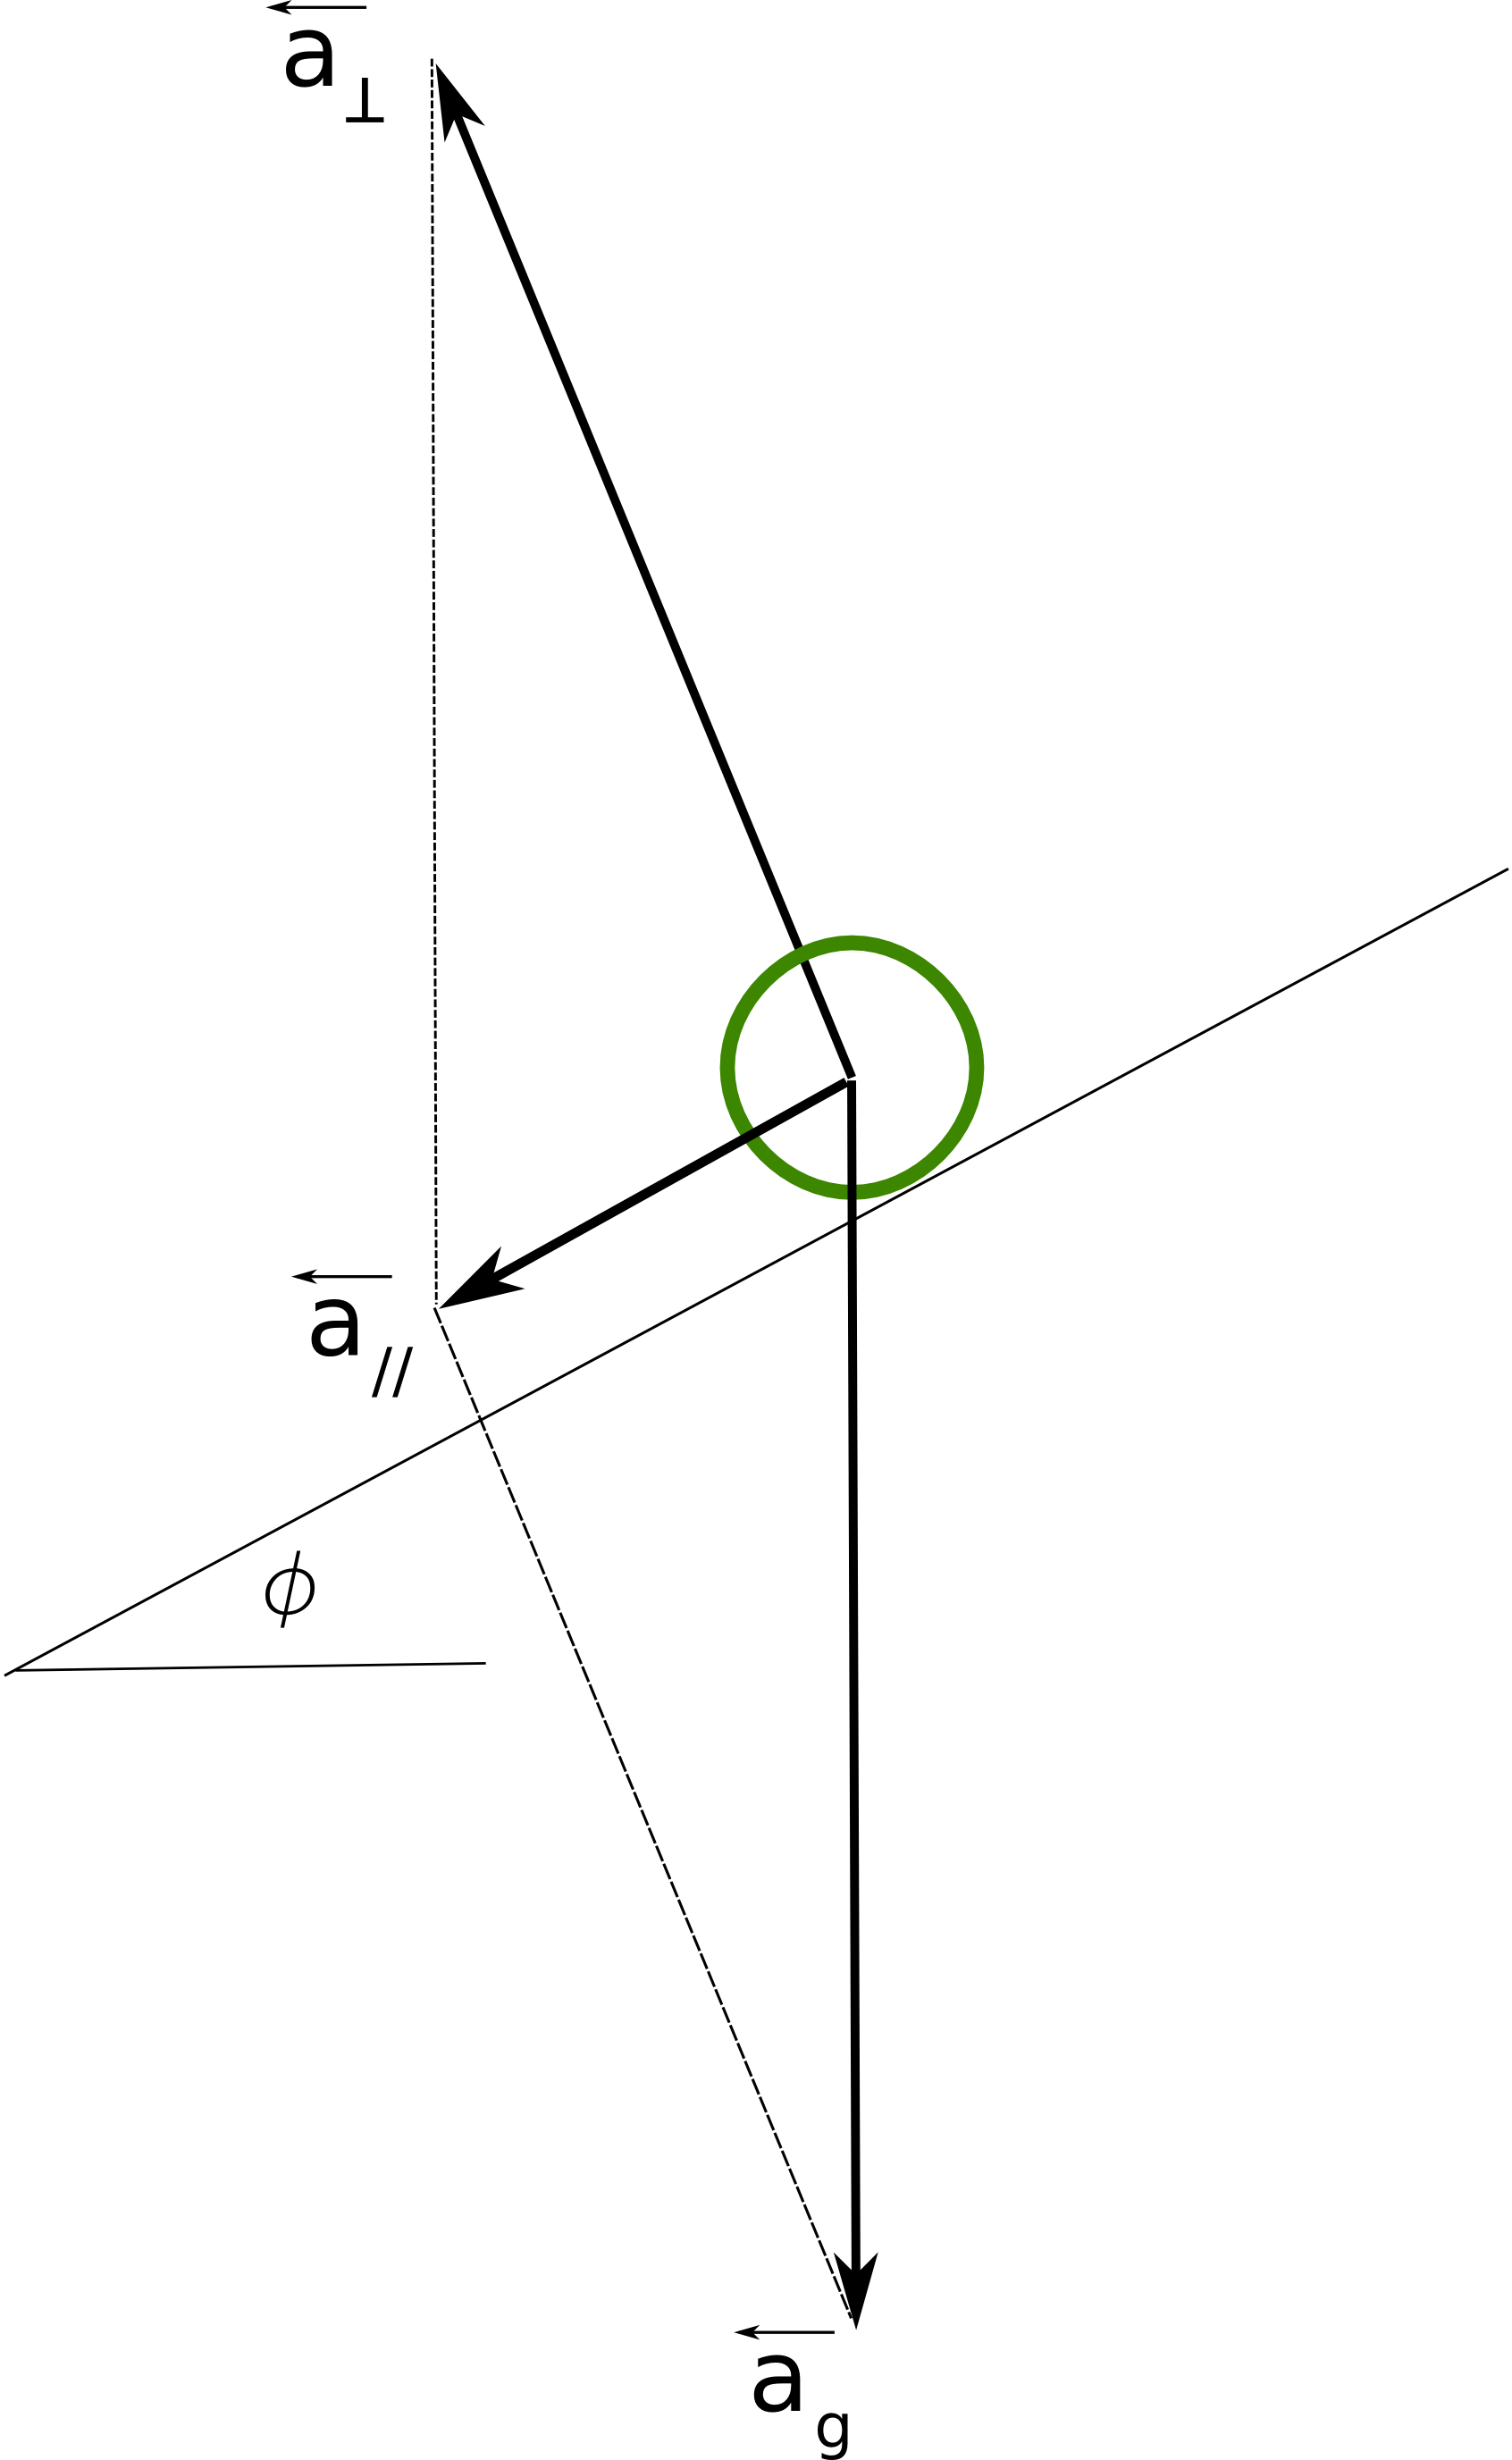
\includegraphics[width=.3\textwidth]{../immagini/gravitaEvincolo.png}
 \label{fig:gravita e reazione vincolare}
\end{figure}

come si può vedere, la relazione tra le accelerazioni in gioco dipende dall'inclinazione $\phi$ del piano, e risulta:

\begin{center}
\begin{math}
\left\{
\begin{array}{r}
a_{//} = a_g sen \phi \\
a_{\perp} = a_g cos \phi
\end{array}
\right.
\end{math}
\end{center}


\subsubsection*{Il coefficiente di attrito}

La seconda forza che agisce sul cilindro che rotola è l'attrito. Questa forma di attrito è detta attrito volvente, perché ha la funzione di far ruotare il cilindro su se stesso e, al medesimo tempo, di rallentarne la corsa.\newline

L'attrito tra due corpi è tanto maggiore quanto più essi sono compressi l'uno contro l'altro, e viene pertanto confrontato con la forza di reazione vincolare esercitata dal piano inclinato sul cilindro mobile. Si definisce pertanto come coefficiente d'attrito il rapporto:

\begin{center}
\begin{equation}
\mi = \frac {a_a}{a_{perp}}
\end{equation}
\end{center}

\subsubsection*{L'inclinazione del piano}

Se abbiamo capito abbastanza bene il fenomeno dello scivolamento della pila, dovremmo essere in grado di impostare e risolvere un esercizio di questo tipo:\newline

{\bf Testo:}
Un mobile scivola su un piano in clinato con accelerazione costante sia in discesa che in salita, ma in discesa l'accelerazione vale $2.74 m/{s^2*}$, mentre in salita vale $9.02 {m/s}$.

Calcolare l'inclinazione del piano e il coefficiente d'attrito.\newline

{\bf Soluzione}
Il problema può essere rappresentato dalla figura qui sotto, che abbiamo già ossevato in precedenza.

\begin{figure}[H]
 \centering
 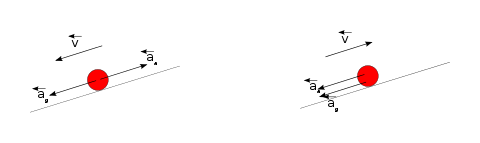
\includegraphics[width=.7\textwidth]{../immagini/leCauseDelMotoDellaPila.png}
 \label{fig:causeDelMotoDellaPila}
\end{figure}

Dai dati del problema definiamo $a_d = 9.02 m/{s^2}$ l'accelerazione totale in discesa e $a_s = - 2.74 m/{s^2}$ quella del moto di salita. Negativa per sottolineare la direzione opposta a quella precedente.

Osservando la figura si può scrivere:
\begin{center}
\begin{equation}
\left\{
\begin{array}{r}
a_s = a_{//} + a_a \\
a_d = a_{//} - a_a
\end{array}
\right.
\end{equation}
\end{center}

In questo sistema, $a_{//}$ e $a_a$ sono due incognite che possono essere risolte sommando e sottraendo membro a membro:\newline

\begin{center}
\begin{math}
\left\{
\begin{array}{r}
a_{//} = \frac{1}{2} a_s + a_d = 5.88 m/{s^2} \\
a_a = \frac{1}{2} a_s - a_d = 3.14 m/{s^2}
\end{array}
\right.
\end{math}
\end{center}

L'accelerazione verso il basso $a_g$ dipende dalla gravità e dall'inclinazione del piano, che può determinata in questo modo:
\newline

\begin{math}
sen \vartheta = \frac{a_{||}}{g} = \frac{5.88\ m/s^2}{9.8\ m/s^2} = 0.60 \\
\end{math}
\begin{math}
\vartheta = arcsen\ 0.60 = 0.64\ rad = 36.9° 
\end{math}

A questo punto è possibile calcolare il coefficiente di attrito. Prima di tutto, dobbiamo cercare l'accelerazione vincolare, che è un cateto del triangolo rettangolo formato con la gravità e l'accelerazione parallela:\newline

\begin{math}
a_{\perp} = \sqrt{g_2 - a_{a}} = \sqrt{9.8^2 - 5.88^2} = 7.84 m/s^2
\end{math}

\begin{math}
\mu = \frac {a_a}{a_\perp} = \frac{3.14}{7.84} = 0.4
\end{math}

\end{document}
